\documentclass{article}
\usepackage[ngerman]{babel}
\usepackage[utf8]{inputenc}
\usepackage{graphicx} 
\usepackage{svg}
\usepackage{listings}
\usepackage{color}
\graphicspath{{img/}}
\usepackage{geometry}
\geometry{a4paper, top=25mm, left=30mm, right=25mm, bottom=20mm}
\usepackage{acronym}
\lstset{
   basicstyle=\scriptsize\ttfamily,
   keywordstyle=\bfseries\ttfamily\color{orange},
   stringstyle=\color{green}\ttfamily,
   commentstyle=\color{middlegray}\ttfamily,
   emph={square}, 
   emphstyle=\color{blue}\texttt,
   emph={[2]root,base},
   emphstyle={[2]\color{yac}\texttt},
   showstringspaces=false,
   flexiblecolumns=false,
   tabsize=2,
   numbers=left,
   numberstyle=\tiny,
   numberblanklines=false,
   stepnumber=1,
   numbersep=10pt,
   xleftmargin=15pt
}

\begin{document}

\tableofcontents
\newpage
\section*{Abkürzzungsverzeichnis}
\begin{acronym}[Bash]
\acro{TLC}{Target Language Compiler}
\acro{STF}{System Target File}
\acro{TMF}{Template Makefile}
\end{acronym}

\newpage
\section{Einführung}
Der Inhalt dieser Dokumentation besteht darin, die Umsetzung von eigenen SW-Treiber für eine Microcontroller-Plattform in Simulink zu erläutern. Hierfür wird zuerst die allgemeine Funktionsweise und insbesondere der Codegenerationsprozess mit Simulink diskutiert. Im Anschluss wird eine Übersicht über die verschiedenen Möglichkeiten dargestellt um eigene Simulink-Blöcke zu erstellen und in Quellcode zu übersetzen. MathoWorks sowohl Online- als auch PDF-Dokumentationen zur Verfügung, auf welche auch durchgehend verwiesen wird.

\newpage
\section{Funktionsweise von Simulink}
Simulink ist eine auf Blockschaltbildern basierende Programmierplattform, welche ursprünglich dazu gedacht war Differentialgleichungen numerisch zu lösen und Simulationen durchzuführen. Im Verlauf der Zeit wurde diese Basis kontinuierlich erweitert und unterstützt mittlerweile zahlreiche Funktionen. Eine bemerkenswerte Funktionalität von Simulink ist die Generation von Quellcode für Microcontroller. Damit können sowohl in kurzer Zeit umfangreiche Applikationen entworfen werden als auch durch Kommunikationsprotokolle zwischen Host- und Target-Plattform HiL-, SiL- und PiL-Simulationen durchgeführt werden. Somit stellt es ein mächtiges Werkzeug dar um Hardwarebausteine wie Sensoren und Microcontroller auszuwerten und daraufhin Filter und Regelungssysteme zu entwerfen.

In den folgenden Abschnitten werden die verschiedenen Ausführungsmodi und der Simulationsprozess von Simulink näher erklärt.

\subsection{Ablauf einer Simulink-Simulation}
Der Ablauf einer Simulation läuft in verschiedenen Phasen ab. Zuerst wird ein Model initialisiert. Hierbei werden die Datentypen, Weiten und Abtastraten der Blöcke und Signale festgelegt. Anschließend werden die Blockparameter ausgewertet und die Blockreihenfolge zur Ausführung bestimmt. Im nächsten Schritt wird die Simulation in einer Schleife ausgeführt. Das einmalige durchlaufen dieser Schleife wird auch als Simulationsschritt (Simulation step) bezeichnet. Der Aufbau der Simulationsschleife hängt von den Eigenschaften des Modelles ab. Besitzt ein Simulink-Modelle Blöcke mit variablen Abtastraten wird vor jedem Simulationsschritt dessen Ausführungszeitpunkt berechnet. Bei einem Modell fixen Abtastraten wird diese Berechnung nicht benötigt. Außerdem wird zwischen Blöcken mit diskreten und kontinuierlichen Zuständen unterschieden. Ein Block mit diskreten Zuständen wird einmal pro Simulationsschritt aufgerufen um seinen, für diesen Simulationsschritt, aktuellen Zustand und Ausgangswerte zu berechnen. Bei einem Block mit kontinuierlichen Zuständen wird dieser mit einer höheren Abtastrate als das restliche Model aufgerufen. In diesen Aufrufen werden die aktuellen Ausgangswerte und Ableitungen des Blocks berechnet.

\begin{figure}[h]
	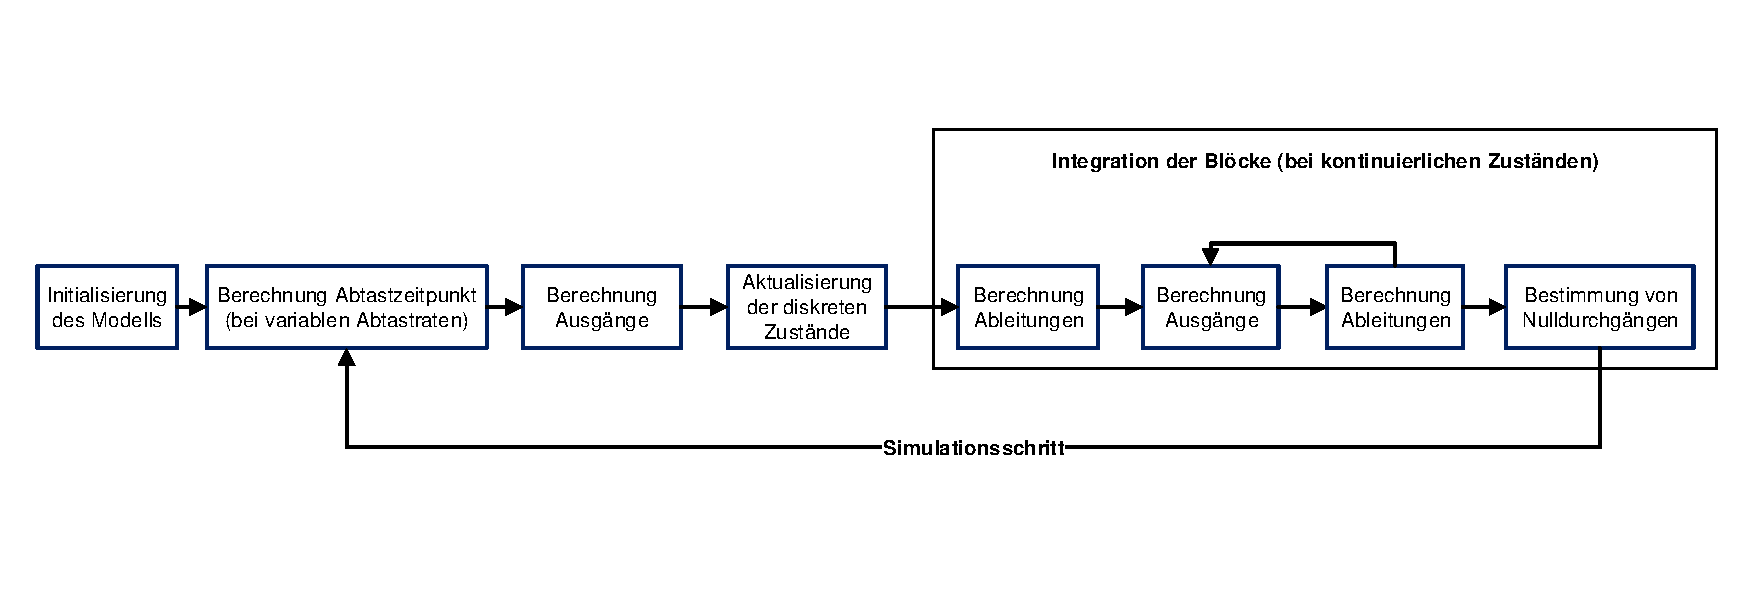
\includegraphics[width=\linewidth]{AblaufSimulation}
	\caption{Ablauf einer Simulation, Quelle: eigene Darstellung, Inhalt aus \cite{SFunc}}
\end{figure}

\subsection{Codegeneration mit Simulink}
Simulink bietet neben der Standardausführung eines Modell auch die Generation von Quellcode, der sowohl auf der Host- als auch auf anderen Zielplattformen ausgeführt werden. Die hierfür benötigten Produkte sind \textit{Simulink-Coder}\footnote{Früher als Real-Time-Workshop bekannt, deshalb wird in vielen Quellen nach wie vor von dem Real-Time-Workshop bzw. RTW gesprochen.} als Basis und ggf. \textit{Embedded-Coder}, welcher die Generation von optimierten C/C++-Code für Microcontroller-Plattformen ermöglicht. Die folgenden Abschnitte stellen den Ablauf einer Codegenration für Modelle mit einfachen, fixen Abtastraten vor. Für weitere Details über die Codegeneration von komplexen Modellen, welche beispielsweise variable Abtastraten, kontinuierliche Zustände und asynchrone Scheduling-Strategien verwenden, sei auf \cite{SimCoder} und \cite{EmbCoder}.

\subsection{Ablauf einer Simulink-Codegeneration}
Der Beginn einer Codegeneration ist identisch mit der üblichen Simulation. Das heißt, dass die Signale, Blockparameter und Abtastraten evaluiert werden. Anschließend legt Simulink die Ausführungsreihenfolge der Blöcke fest. Anschließend erstellt \textit{Simulink-Coder} eine RTW-Datei (.rtw), welche diese Informationen über das Modell enthält. Im nächsten Schritt wird die RTW-Datei dem \ac{TLC} übergeben, welcher die Generation des Quellcodes durchführt. \ac{TLC} ist eine von TheMathWorks entwickelte Programmiersprache bzw. der Interpreter, welche diese auswertet. Diese Programmiersprache ermöglicht einerseits die Auswertung von RTW-Dateien, andererseits können auch Code-Datein in beliebigen Sprachen erstellt werden. Für mehr Informationen über die Funktionsweise und Syntax von \ac{TLC} sei auf \cite{TLC} verwiesen.

Für die Codegeneration benötigt der \ac{TLC} neben der RTW-Datei des Modelles, ein \ac{STF}, ein \ac{TMF}, die Standard-TLC-Bibliothek und die \ac{TLC}-Dateien der einzelnen Blöcke, welche die Vorschrift für die Codegeneration des Blocks enthalten.

\begin{figure}[h]
	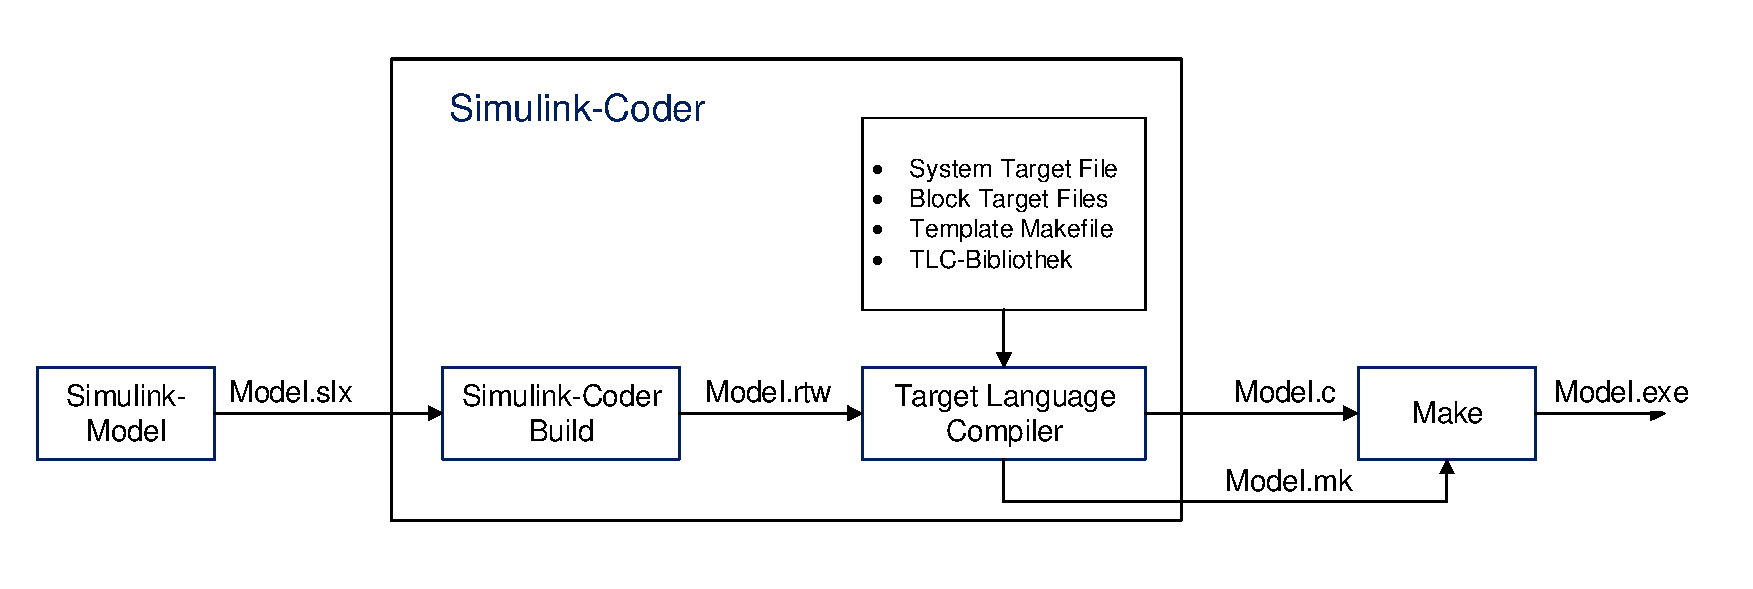
\includegraphics[width=\linewidth]{AblaufCodegeneration}
	\caption{Ablauf Codegeneration, Quelle: eigene Darstellung, Inhalt aus \cite{TLC}}
\end{figure}

\subsubsection{System Target File}
Das \ac{STF} stellt den Ausgangspunkt der \ac{TLC}-Codegeneration dar. In dieser Datei werden zuerst die Grundeinstellungen, wie z.B. das Codeformat und die Programmiersprache festgelegt. Anschließend werden eigenen Simulink-Blöcken TLC-Dateien zugeordnet, welche die Generationsvorschriften enthalten. Im nächsten Schritt wird die Ausführung der Simulink-Blöcke in entsprechender Reihenfolge in Quellcode übersetzt. Hierfür wird in der Regel die Datei "codegenentry.tlc" verwendet, welche von Simulink bereitgestellt wird. Diese Datei ordnet den Standard-Blöcken die entsprechenden TLC-Dateien zu, initialisiert globale Variablen und führt die Codegeneration eines einzelnen Simulationsschrittes durch. Zuletzt wird eine TLC-Datei inkludiert, welche eine main-Datei erstellt. In der main-Routine werden ggf. allgemeine Ressourcen initialisiert und die Simulationsschritte, den Abtastraten entsprechenden, aufgerufen.

\subsubsection{Template Make File}
Der \ac{TLC} erzeugt bei der Codegeneration ein Makefile um den Quellcode in ein ausführbares Format zu übersetzen. Das Makefile wird von einem \ac{TMF} abgeleitet, in welchem unter anderem die Toolchain, zusätzliche Bibliotheken und Compiler-Einstellungen festgelegt werden. Somit ermöglicht es ein \ac{TMF} auch Modelle auf beliebigen Zielplattform auszuführen, insofern eine Cross-Compiler-Toolchain zur Verfügung steht.

\newpage
\section{Aufbau und Implementierung von Simulink-Blöcken}
Ein Simulink-Block muss Funktionen bereitstellen um die einzelnen Schritte einer Simulation zu ermöglichen. Darunter fallen die Folgenden Funktionen:

\begin{itemize}
	\item Initialisierung des Blocks
	\item Berechnung des nächsten Abtastzeitpunktes (falls der Block variable Abtastraten benötigt)
	\item Berechnung der Ausgangswerte
	\item Berechnung der diskreten Zustände des Blocks
	\item Integration, hierunter fallen die Berechnung der Ausgangswerte und Ableitungen bei Zwischenschritten (wird nur bei kontinuierlichen Zuständen benötigt)
\end{itemize}

Die Umsetzung dieser Methoden erfolgt in der Form einer sogenannten \textit{S-Function}. Hierbei handelt es sich lediglich um eine Sammlung von Funktionen, welche die oben genannten Aktionen implementieren. Eine \textit{S-Function} kann in unterschiedlichen Programmiersprachen implementiert werden, wobei MATLAB und C/C++ die üblichsten sind. Hier sollen lediglich \textit{S-Functions} in C/C++ vorgestellt werden, in \cite{SFunc} werden alle Alternativ detailliert erklärt. 

\subsection{C/C++ S-Function}
In diesem Abschnitt wird der Aufbau einer \textit{S-Function} am Beispiel eines einfachen Blocks, der seinen Eingang mit einem fixen Wert multipliziert, erklärt. Dieser Block benötigt keine kontinuierlichen Zustände, somit müssen lediglich Funktionen zur Initialisierung, Berechnung der Ausgänge und Terminierung am Ende der Simulation implementiert werden.

\begin{figure}[h]
\label{CustomGain_Overview_pic}
	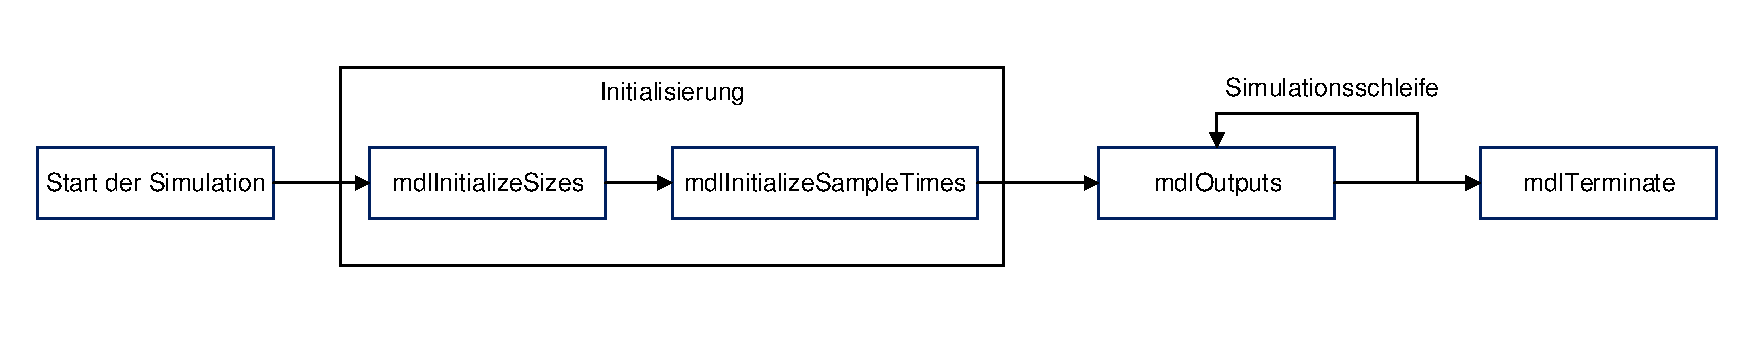
\includegraphics[width=\linewidth]{CustomGain_Overview}
	\caption{Interaktion eines diskreten Block mit der Simulink-Engine, Quelle: eigene Darstellung, Inhalt aus \cite{SFunc}}
\end{figure}

Die Implementierung in C++ beginnt mit der Definition der des Namen und Level der \textit{S-Function}. Das Level einer \textit{S-Function} sollte auf 2 gesetzt werden, bei dem Level 1 handelt es sich um einen veralteten \textit{S-Function} Typ. Außerdem werden die benötigten Header-Dateien inkludiert.

\begin{lstlisting}
#define S_FUNCTION_NAME CustomGain_SFunction
#define S_FUNCTION_LEVEL 2

#include "simstruc.h"
#include "matrix.h"
\end{lstlisting}

Anschließend werden die in \ref{CustomGain_Overview_pic} dargestellten Funktionen implementiert. Die Funktion \textit{mdlInitializeSizes} legt die Anzahl der Parameter, Ein- und Ausgänge fest. Anschließend werden die Weiten der Ein- bzw. Ausgangssignale eingestellt und die Anzahl der Abtastraten festgesetzt. Hierfür wird das s.g. \textit{SimStruct} verwendet. Hierbei handelt es sich um eine Baumstruktur, welche die Informationen über das gesamte Model und Blöcke enthält. Die Wurzel des \textit{SimStruct} ist das gesamt Modell, welches in die verschiedenen Subsysteme und Blöcke verzweigt. Die \textit{SimStruct}-Referenz die den Funktionen einer \textit{S-Function} übergeben wird, verweist auf das jeweilige Blatt der Baumstruktur, welche den Block repräsentiert.

\begin{lstlisting}
static void mdlInitializeSizes(SimStruct* S)
{
    //Anzahl der S-Function Parameter festlegen
    ssSetNumSFcnParams(S,1);         
    if(ssGetNumSFcnParams(S) != ssGetSFcnParamsCount(S)) return;
    
    //Anzahl der Eingaenge und deren Weite festlegen und ueberpruefen
    if(!ssSetNumInputPorts(S,1)) return;
    ssSetInputPortWidth(S, 0, 1);
    ssSetInputPortDirectFeedThrough(S, 0, 1);
    
    //Anzahl der Ausgaenge und deren Weite festlegen
    if(!ssSetNumOutputPorts(S,1)) return;
    ssSetOutputPortWidth(S, 0, DYNAMICALLY_SIZED);
    
    //Anzahl der Abtastsraten festlegen
    ssSetNumSampleTimes(S, 1);
}
\end{lstlisting}

In der Initialisierungsphase müssen außerdem die Abtastraten spezifiziert werden. Dies geschieht in der Funktion \textit{mdlInitializeSampleTimes}. Der Wert \textit{INHERITED\_SAMPLE\_TIME} bedeutet, dass die Abtastrate der Blöcke, welche das Ausgangssignal erhalten, übernommen wird.

\begin{lstlisting}
static void mdlInitializeSampleTimes(SimStruct* S)
{
    //Festelegen der Abtastrate und Abtastoffset auf INHERITED
    ssSetSampleTime(S, 0, INHERITED_SAMPLE_TIME);
    ssSetOffsetTime(S, 0, 0.0);
}
\end{lstlisting}

Während der Simulation ruft die Simulink-Engine die \textit{mdlOutputs} Funktion auf um den Ausgangswert des Blocks zu ermitteln. In diesem Fall wird der Eingangswert mit dem Block-Parameter multipliziert.

\begin{lstlisting}
static void mdlOutputs(SimStruct* S, int_T tid)
{   
    //Eingang-, Ausgangsignale und Parameter von dem SimStruct abfragen
    InputRealPtrsType inputPtrArr  = ssGetInputPortRealSignalPtrs(S, 0);
    real_T* outputPtr              = ssGetOutputPortRealSignal(S, 0);
    const mxArray* parameterPtr    = ssGetSFcnParam(S, 0);
    //Ausgangswert berechnen
    *outputPtr = (*(inputPtrArr[0])) * (*mxGetPr(parameterPtr));
}
\end{lstlisting}

Am Ende der Simulation wird die \textit{mdlTerminate} Funktion ausgeführt. Hier müssen ggf. reservierte Ressourcen wieder freigeben werden.

\begin{lstlisting}
static void mdlTerminate(SimStruct* S)
{
}
\end{lstlisting}

Am Schluss der C++-Datei befinden sich weitere Präprozessordirektiven, welche für die Codegeneration und MEX-Compilation benötigt werden. Diese beiden Ausführungsmodi werden in einem späteren Abschnitt näher erläutert.

\begin{lstlisting}
#ifdef MATLAB_MEX_FILE
#include "simulink.c"
#else
#include "cg_sfun.h"
#endif
\end{lstlisting}

\subsection{Codegeneration einer S-Function}
Eine \textit{S-Function} kann auch in Quellcode übersetzt werden. Die einfachste Form besteht in einer s.g. \textit{non-inlined S-Function}, die darin besteht, dass die C/C++-Datei der \textit{S-Function} direkt als Quelldatei verwendet wird. Somit muss allerdings das komplette \textit{SimStruct} in Quellcode übersetzt werden und den \textit{S-Function} während der Ausführung übergeben werden, wodurch die Größe und Ausführungszeit des Modelles erhöht wird. 

Mit Hilfe von TLC-Dateien kann eine \textit{S-Function} effizient in Quellcode übersetzt werden. In der TLC-Datei werden die Vorschriften festgehalten, wie die Ausgangswerte und Zustände eines Blocks in der gewählten Programmiersprache berechnet werden. Der folgende Codeausschnitt zeigt die \ac{TLC}-Implementation der bereits gezeigten Gain-\textit{S-Function}.

\begin{lstlisting}
%implements "CustomGain_SFunction" "C"

%function Outputs(block, system) Output
    %assign gainFactor  = LibBlockParameter(0, "", "", 0)
    %assign inputValue  = LibBlockInputSignal(0, "", "", 0)
    %assign outputValue = LibBlockOutputSignal(0, "", "", 0)
    %<outputValue>      = %<inputValue> * %<gainFactor>
%endfunction
\end{lstlisting}

Für den Quellcode muss lediglich die Output-Funktion generiert werden, in welcher das Eingangsignal mit dem Wert des Blockparameter multipliziert wird. Auf die Syntax und Funktionalität von \ac{TLC} wird hier nicht näher eingegangen, da Simulink mehrere Werkzeuge zur Verfügung stellt, die es ermöglichen \textit{S-Functions} und die zugehörigen TLC-Dateien automatisch zu erzeugen. Diese werden in den nächsten Abschnitt genauer erklärt.

\subsection{Kompilierung einer S-Function}
C/C++ \textit{S-Functions} müssen in MEX-Dateien übersetzt werden, damit sie in Simulink verwendet werden können. Matlab kann hierfür verschiedene Compiler wie z.B. \textit{MinGW} oder \textit{GCC} verwenden. Eine C/C++ Quelldatei kann über die Matlab Konsole mit dem folgenden Befehl in eine MEX-Datei übersetzt werden.

\begin{lstlisting}
mex CustomGain_SFunction.cpp
\end{lstlisting}

Matlab wählt hier automatisch den Compiler, welcher der Dateiendung entspricht. In dem Fall, das mehrere MEX-kompatible Compiler installiert sind, kann mit dem folgenden Befehl der gewünschte Compiler ausgewählt werden.

\begin{lstlisting}
mex -setup myCompiler
\end{lstlisting}

Die Verwendung von TLC-Dateien zur Codegeneration einer \textit{S-Function} bringt hier weitere Vorteile mit sich. Da eine \textit{non-inlined S-Function} ihre C/C++-Quelldatei sowohl für die MEX- als auch Target-Kompilierung verwendet wird, muss mit Hilfe von Makros der Quellcode geteilt werden. Der erste Teil dient als Quelle für die MEX-Datei. Der zweite Teil wird für die generierte Datei verwendet.

\begin{lstlisting}
#ifdef MATLAB_MEX_FILE
	/* Quellcode fuer die MEX-Datei */
#else
	/* Quellcode fuer die Zielplattform */
#endif
\end{lstlisting}

Dadurch ensteht eine unnötig große und unübersichtliche Quelldatei. Bei der Verwendung einer TLC-Datei wird die C/C++-Quelle lediglich für die MEX-Kompilierung verwendet. Der Quellcode für die Zielplattform-Kompilierung wird mit Hilfe der TLC-Datei kompiliert.

\subsection{S-Function-Builder}
Simulink bietet neben den gewöhnlichen \textit{S-Function}-Blöcken auch einen \textit{S-Function-Builder}-Block. Dieser bietet eine graphische Benutzeroberfläche, welche die Konfiguration einer \textit{S-Function} ermöglicht. Der \textit{S-Function-Builder} erzeugt im Anschluss eine C- und TLC-Datei und kompiliert die MEX-Datei. Dadurch kann die Entwicklung von Simulink-Blöcken stark vereinfacht werden, vor allem da keine TLC-Kenntnisse erforderlich sind.

\newpage
\renewcommand\refname{Literaturverzeichnis}
\begin{thebibliography}{}
	\bibitem{SFunc} TheMathWorks, "Writing S-Functions", März 2016
	\bibitem{TLC} TheMathWorks, "Target Language Compiler", März 2016
	\bibitem{SimCoder} TheMathWorks, "Simulink Coder User Guide", März 2016
	\bibitem{EmbCoder} TheMathWorks, "Embedded Coder User Guide", März 2016
\end{thebibliography}
\end{document}